\subsection{Architettura generale - Componenti del sistema}
\subsubsection{Monolith}
   \FloatBarrier
   \begin{figure}[ht]
   \centering
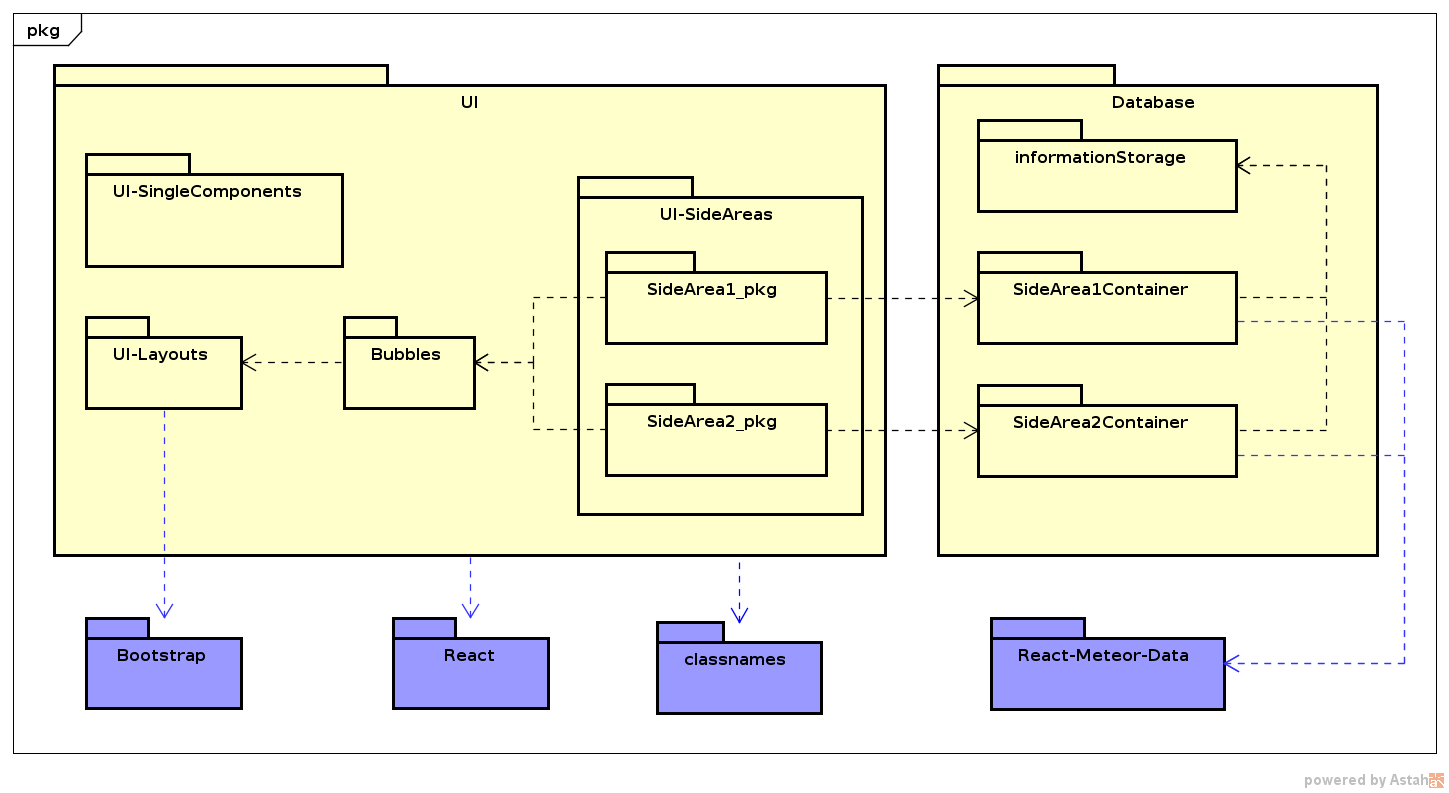
\includegraphics[width=\textwidth,keepaspectratio]{img/General}
   \caption{Diagramma per Monolith.}
\end{figure}
\FloatBarrier
\textbf{Descrizione}:\\
 Componente che rappresenta l'intera SDK di Monolith 


\clearpage

\subsubsection{Monolith::Database}
\textbf{Descrizione}:\\
 Componente contenente i pacchetti che vengono utilizzati per interagire con il database 


\clearpage

\subsubsection{Monolith::Database::InformationStorage}
   \FloatBarrier
   \begin{figure}[ht]
   \centering
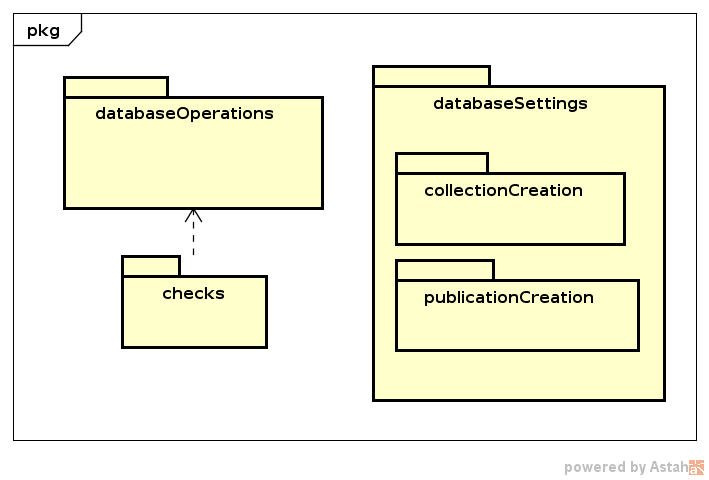
\includegraphics[width=\textwidth,keepaspectratio]{img/informationStorage}
   \caption{Diagramma per Monolith::Database::InformationStorage.}
\end{figure}
\FloatBarrier
\textbf{Descrizione}:\\
 Componente per la configurazione dell'utilizzo del database 


\clearpage

\subsubsection{Monolith::Database::informationStorage::Checks}
   \FloatBarrier
   \begin{figure}[ht]
   \centering
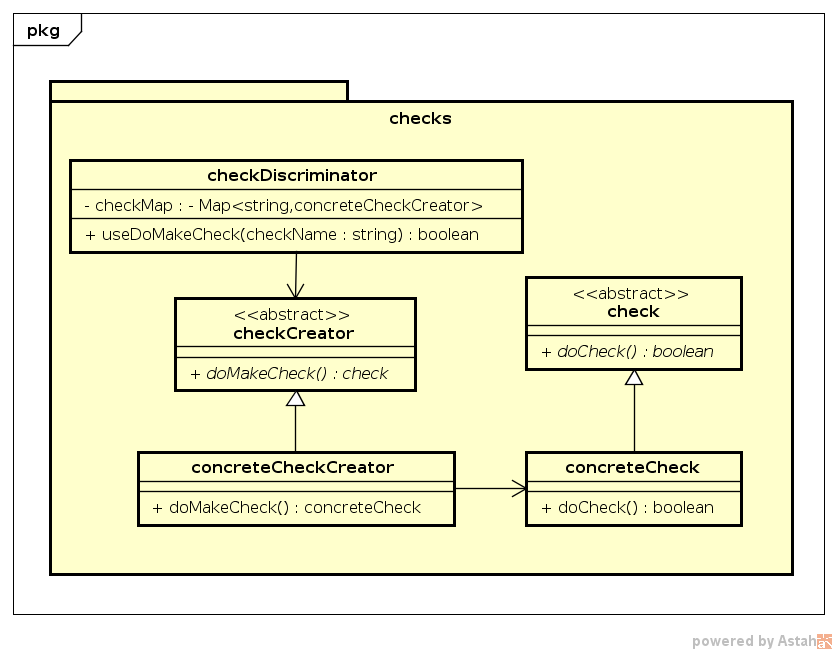
\includegraphics[width=\textwidth,keepaspectratio]{img/controls}
   \caption{Diagramma per Monolith::Database::informationStorage::Checks.}
\end{figure}
\FloatBarrier
\textbf{Descrizione}:\\
 Componente per la creazione dei controlli da effettuare sul client prima di effettuare l'inserimento dei dati nel database 
\\ \textbf{Classi contenute}:\\
\begin{itemize}
\item check
\item checkCreator
\item checkDiscriminator
\item concreteCheck
\item concreteCheckCreator
\end{itemize}


\clearpage

\subsubsection{Monolith::Database::InformationStorage::DatabaseSettings}
\textbf{Descrizione}:\\
 Modulo per la configurazione delle collection 


\clearpage

\subsubsection{Monolith::UI}
\textbf{Descrizione}:\\
 Componente contenente tutti i pacchetti che servono per comporre e gestire la parte visuale dell'applicazione delle bolle
\textbf{Dipendenze}
\begin{itemize}
\item React
\item classNames
\end{itemize} 


\clearpage

\subsubsection{Monolith::UI::Bubbles}
   \FloatBarrier
 %  \begin{sidewaysfigure}[ht]
%\begin{center}
 \makebox[\textwidth][c]{
\rotatebox{90}{
% \centering
\begin{minipage}{0.8\textheight}
   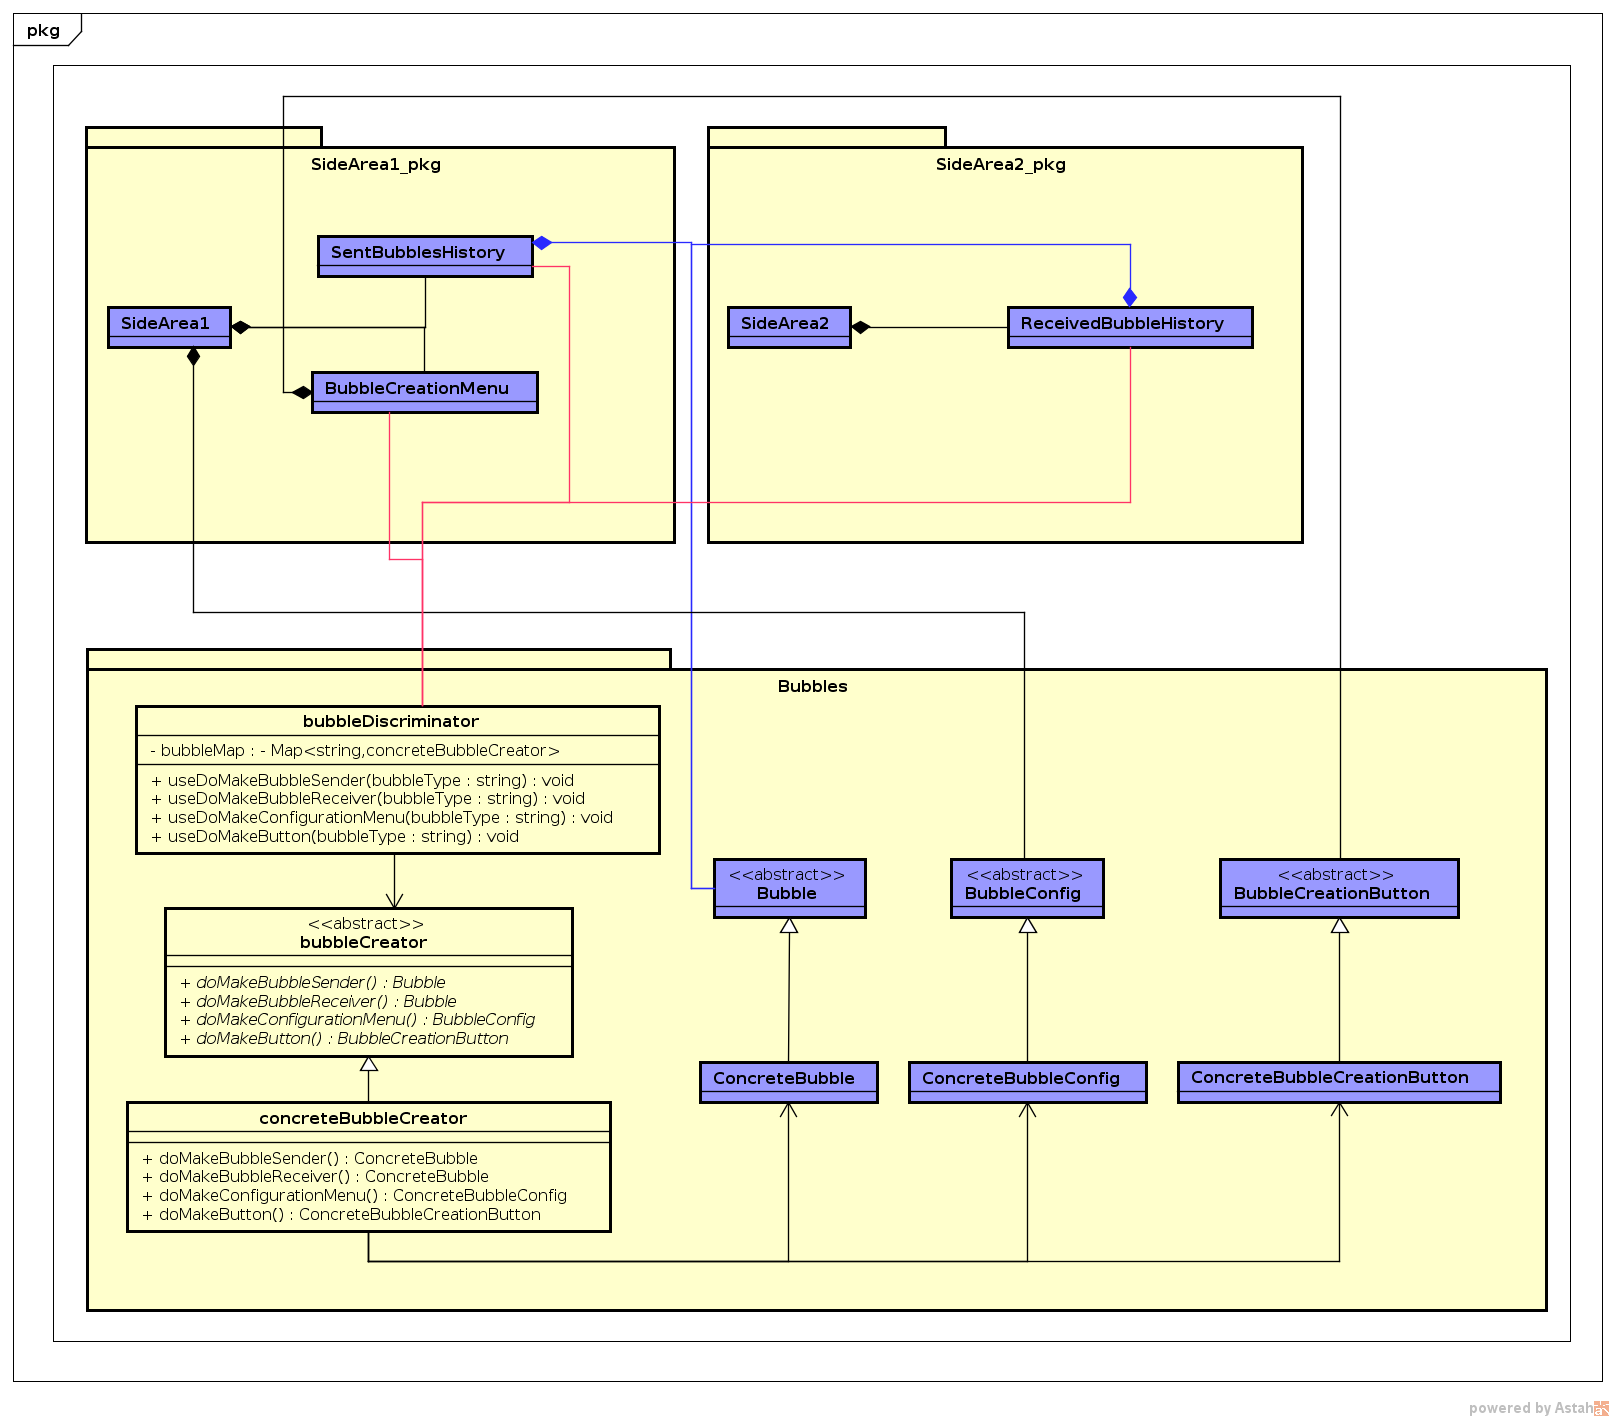
\includegraphics[width=\textwidth,keepaspectratio]{img/Bubbles}
  \captionof{figure}{Diagramma per Monolith::UI::Bubbles.}
\end{minipage}}
}
%\end{center}
%\end{sidewaysfigure}
\FloatBarrier
\textbf{Descrizione}:\\
 Componente per la creazione delle bolle da visualizzare 
\\ \textbf{Classi contenute}:\\
\begin{itemize}
\item Bubble
\item BubbleConfig
\item BubbleCreationButton
\item bubbleCreator
\item bubbleDiscriminator
\item ConcreteBubble
\item ConcreteBubbleConfig
\item ConcreteBubbleCreationButton
\item concreteBubbleCreator
\end{itemize}


\clearpage

\subsubsection{Monolith::UI::SideAreas}
\textbf{Descrizione}:\\
 Contiene i package per la visualizzazione delle bolle nelle side-bar 


\clearpage

\subsubsection{Monolith::UI::SideAreas::SideArea1\_pkg}
\textbf{Descrizione}:\\
 Componente per la visualizzazione delle bolle inviate e del menù di creazione delle bolle nella prima side-bar 
\\ \textbf{Classi contenute}:\\
\begin{itemize}
\item BubbleCreationMenu
\item SentBubbleHistory
\item SideArea1
\end{itemize}


\clearpage

\subsubsection{Monolith::UI::SideAreas::SideArea2\_pkg}
\textbf{Descrizione}:\\
 Componente per la visualizzazione delle bolle ricevute nella seconda side-bar 
\\ \textbf{Classi contenute}:\\
\begin{itemize}
\item ReceivedBubbleHistory
\item SideArea2
\end{itemize}


\clearpage

\subsubsection{Monolith::UI::UI-Layouts}
   \FloatBarrier
   \begin{figure}[ht]
   \centering
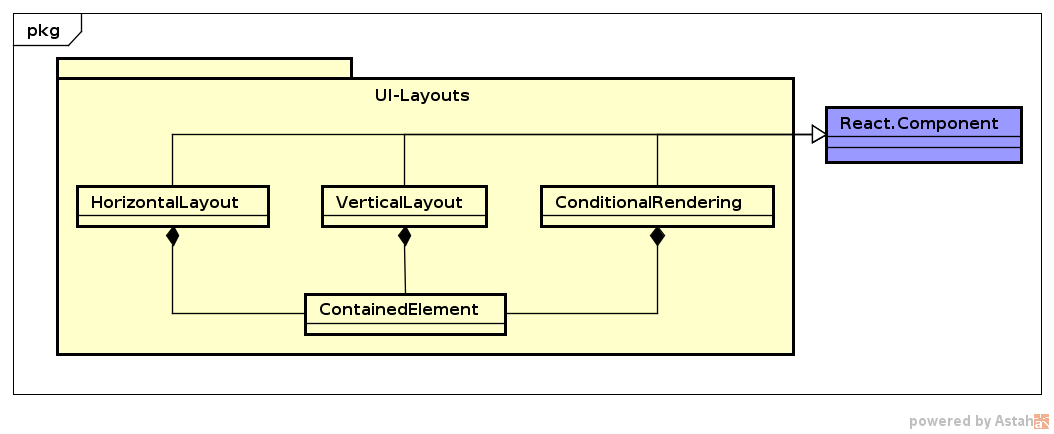
\includegraphics[width=\textwidth,keepaspectratio]{img/UI-Layouts}
   \caption{Diagramma per Monolith::UI::UI-Layouts.}
\end{figure}
\FloatBarrier
\textbf{Descrizione}:\\
 Componente che contiene le classi React per la gestione dei layout
\textbf{Dipendenze} \\
Bootstrap 
\\ \textbf{Classi contenute}:\\
\begin{itemize}
\item ConditionalRendering
\item ContainedElement
\item HorizontalLayout
\item VerticalLayout
\end{itemize}


\clearpage

\subsubsection{Monolith::UI::UI-SingleComponents}
   \FloatBarrier
   \begin{figure}[ht]
   \centering
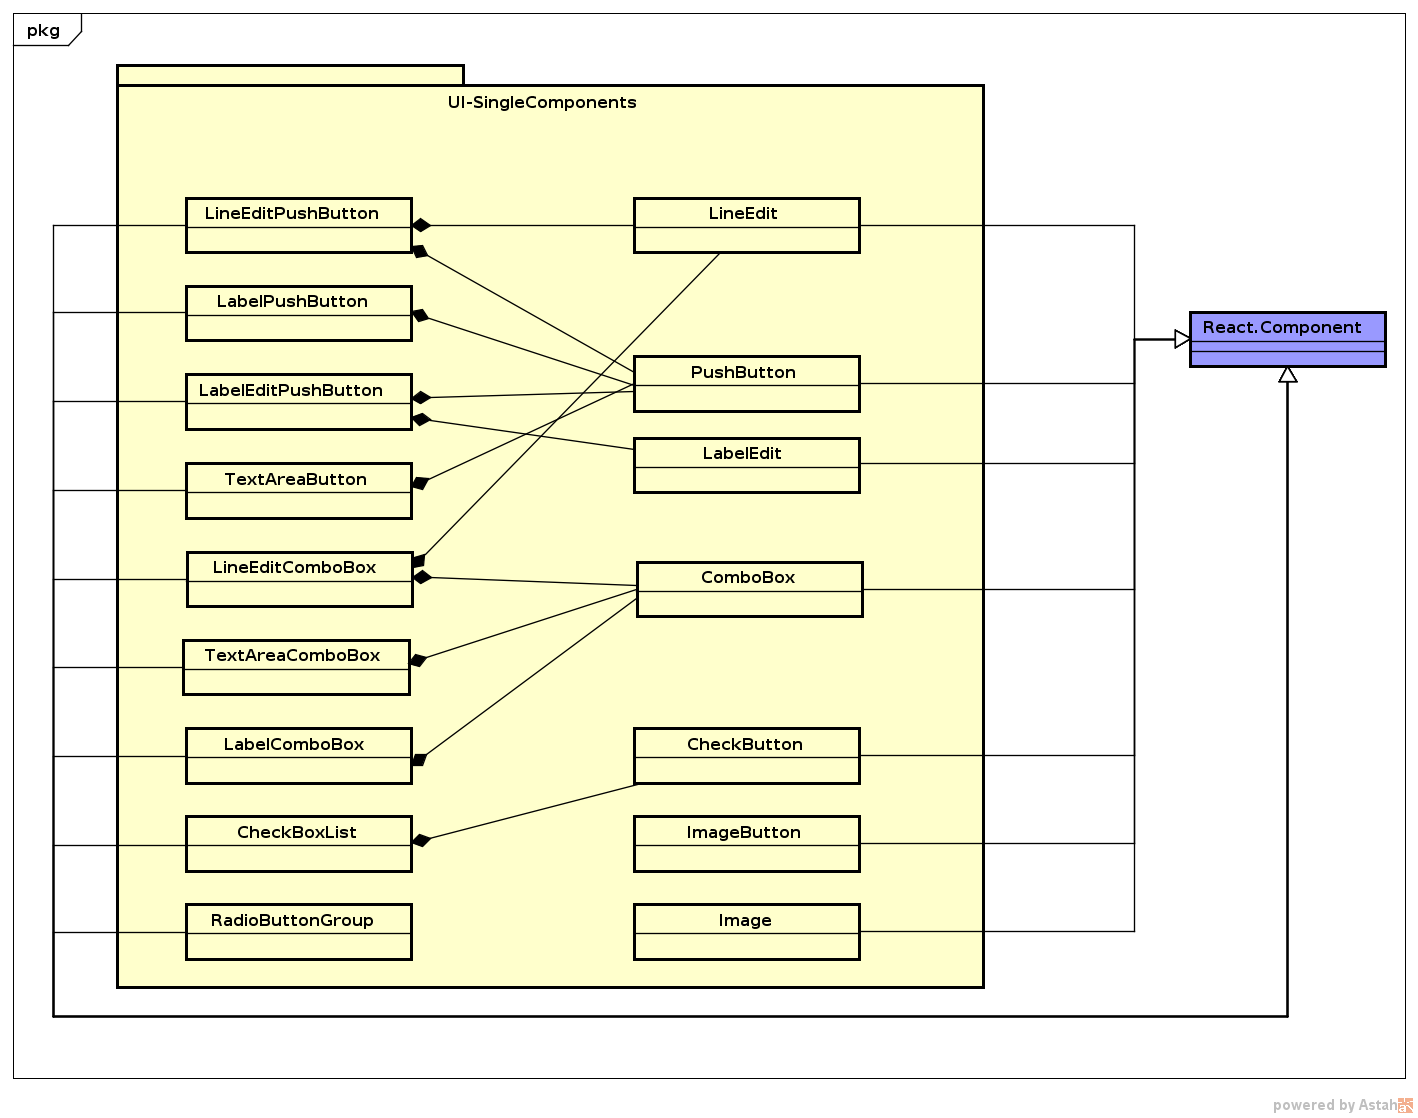
\includegraphics[width=\textwidth,keepaspectratio]{img/UI-SingleComponents}
   \caption{Diagramma per Monolith::UI::UI-SingleComponents.}
\end{figure}
\FloatBarrier
\textbf{Descrizione}:\\
 Componente che contiene tutti i componenti React per la composizione della GUI 
\\ \textbf{Classi contenute}:\\
\begin{itemize}
\item CheckBoxList
\item CheckButton
\item ComboBox
\item Image
\item ImageButton
\item LabelComboBox
\item LabelEdit
\item LabelEditPushButton
\item LabelPushButton
\item LineEdit
\item LineEditComboBox
\item LineEditPushButton
\item PushButton
\item RadioButtonGroup
\item TextAreaButton
\item TextAreaComboBox
\end{itemize}


\clearpage \subsection{Architettura generale - Bolle Demo}
\subsubsection{CurrencyBubble}
   \FloatBarrier
 %  \begin{sidewaysfigure}[ht]
%\begin{center}
 \makebox[\textwidth][c]{
\rotatebox{90}{
% \centering
\begin{minipage}{0.8\textheight}
   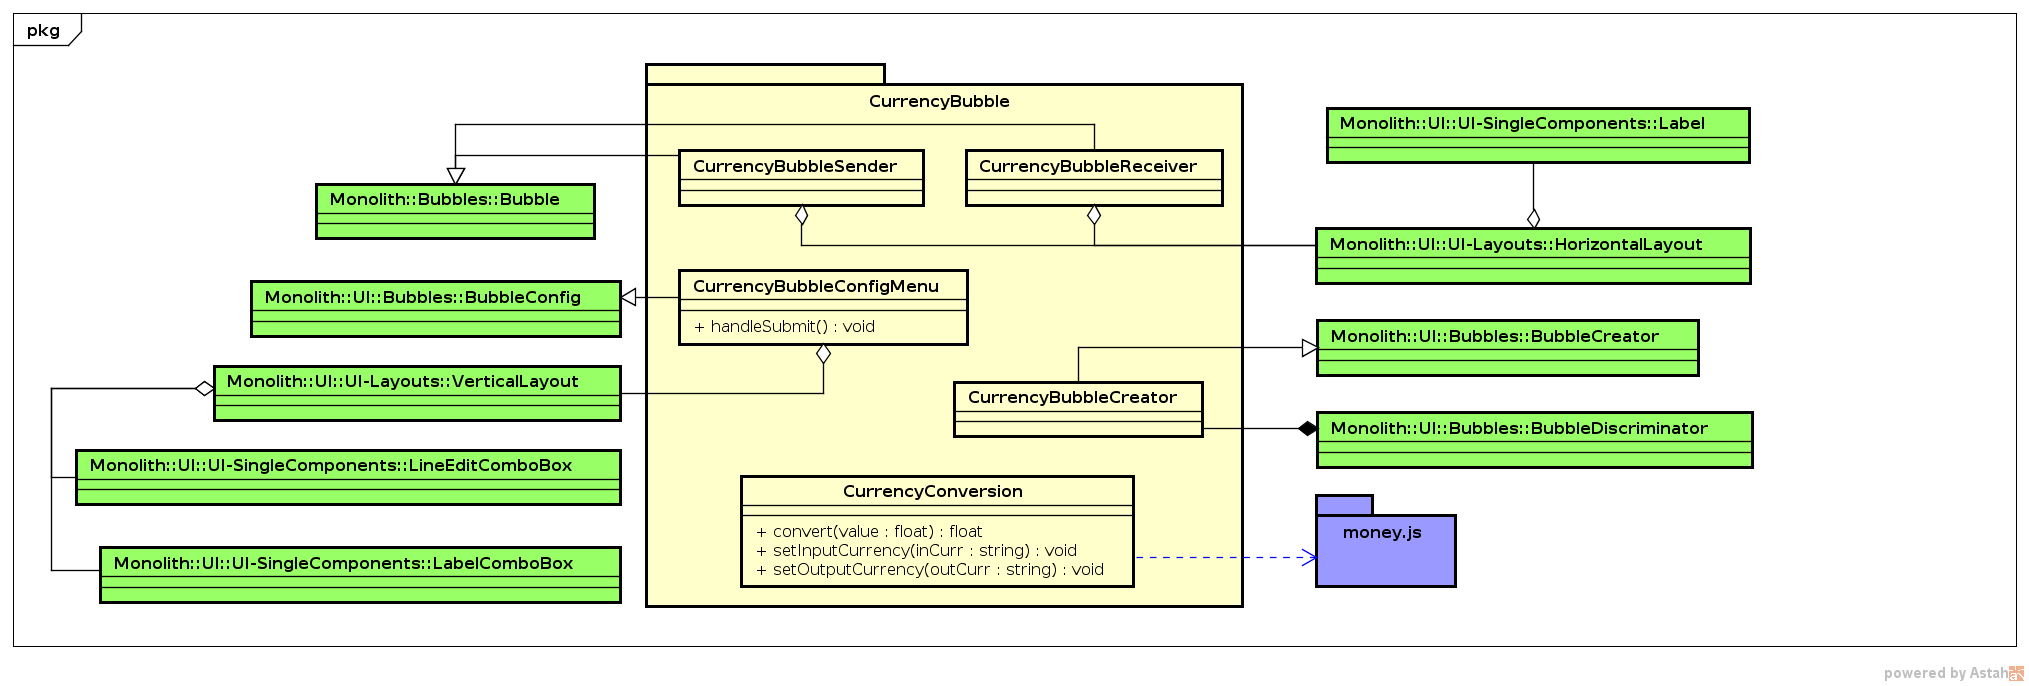
\includegraphics[width=\textwidth,keepaspectratio]{img/currency}
  \captionof{figure}{Diagramma per CurrencyBubble.}
\end{minipage}}
}
%\end{center}
%\end{sidewaysfigure}
\FloatBarrier
\textbf{Descrizione}:\\
 Componente contente le classi necessarie per la creazione della bolla convertitore valute. 
\\ \textbf{Classi contenute}:\\
\begin{itemize}
\item CurrencyBubbleConfigMenu
\item CurrencyBubbleCreator
\item CurrencyBubbleReceiver
\item CurrencyBubbleSender
\item CurrencyConversion
\end{itemize}


\clearpage

\subsubsection{DiceBubble}
   \FloatBarrier
 %  \begin{sidewaysfigure}[ht]
%\begin{center}
 \makebox[\textwidth][c]{
\rotatebox{90}{
% \centering
\begin{minipage}{0.8\textheight}
   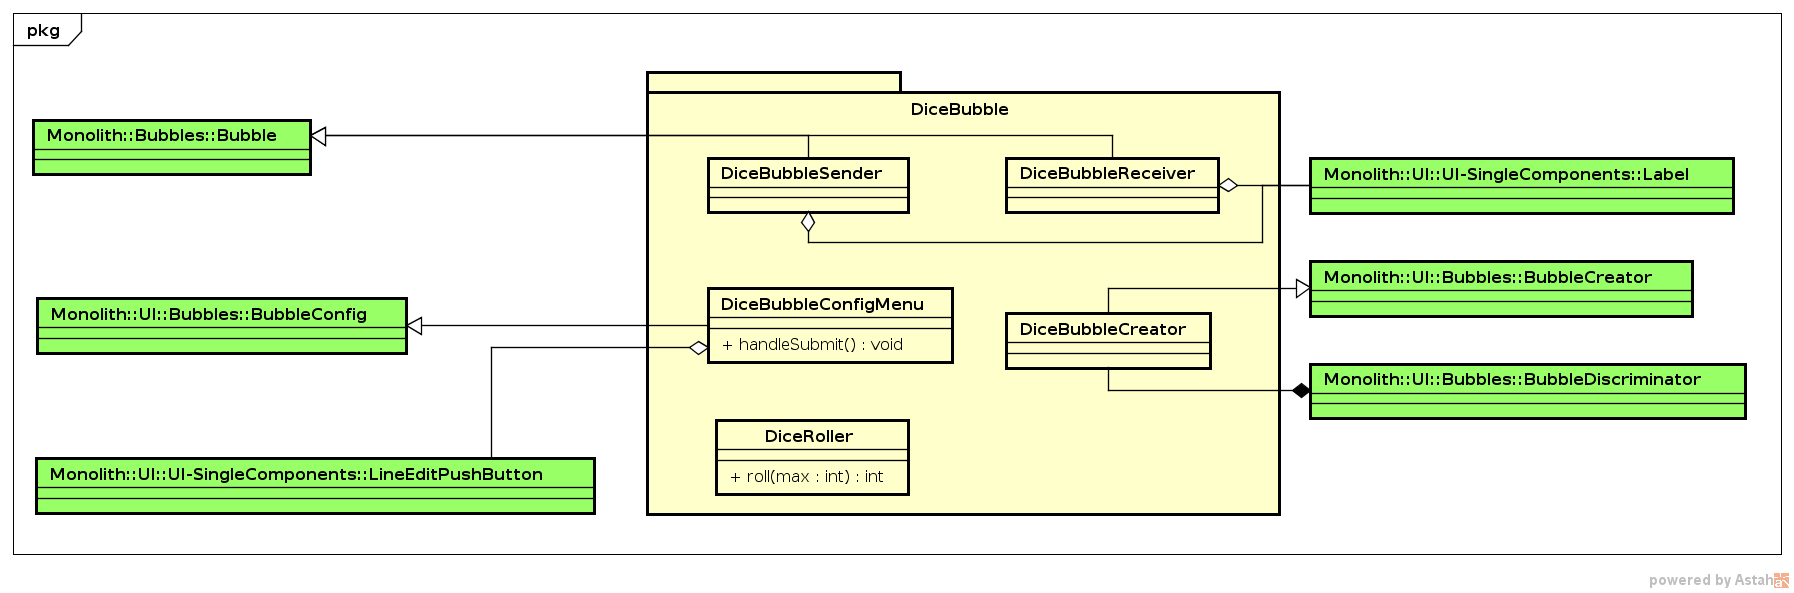
\includegraphics[width=\textwidth,keepaspectratio]{img/dice}
  \captionof{figure}{Diagramma per DiceBubble.}
\end{minipage}}
}
%\end{center}
%\end{sidewaysfigure}
\FloatBarrier
\textbf{Descrizione}:\\
 Componente contente le classi necessarie per la creazione della bolla estrazione numero casuale. 
\\ \textbf{Classi contenute}:\\
\begin{itemize}
\item DiceBubbleConfigMenu
\item DiceBubbleCreator
\item DiceBubbleReceiver
\item DiceBubbleSender
\item DiceRoller
\end{itemize}


\clearpage

\subsubsection{ListBubble}
   \FloatBarrier
   \begin{figure}[ht]
   \centering
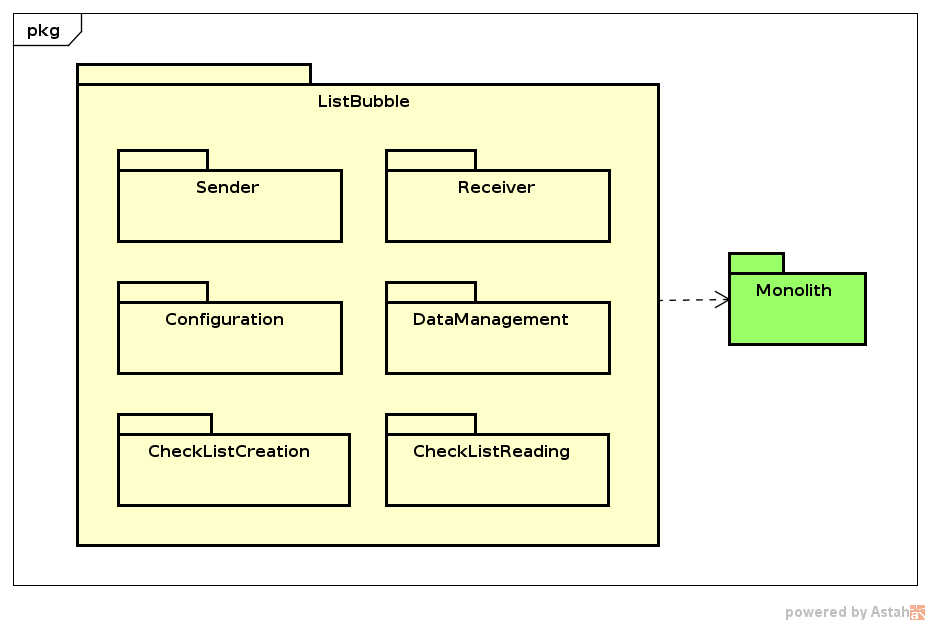
\includegraphics[width=\textwidth,keepaspectratio]{img/listchecklistTop}
   \caption{Diagramma per ListBubble.}
\end{figure}
\FloatBarrier
\textbf{Descrizione}:\\
 Componente contenente i pacchetti necessari per la creazione della bolla lista. 


\clearpage

\subsubsection{ListBubble::CheckListCreation}
   \FloatBarrier
 %  \begin{sidewaysfigure}[ht]
%\begin{center}
 \makebox[\textwidth][c]{
\rotatebox{90}{
% \centering
\begin{minipage}{0.8\textheight}
   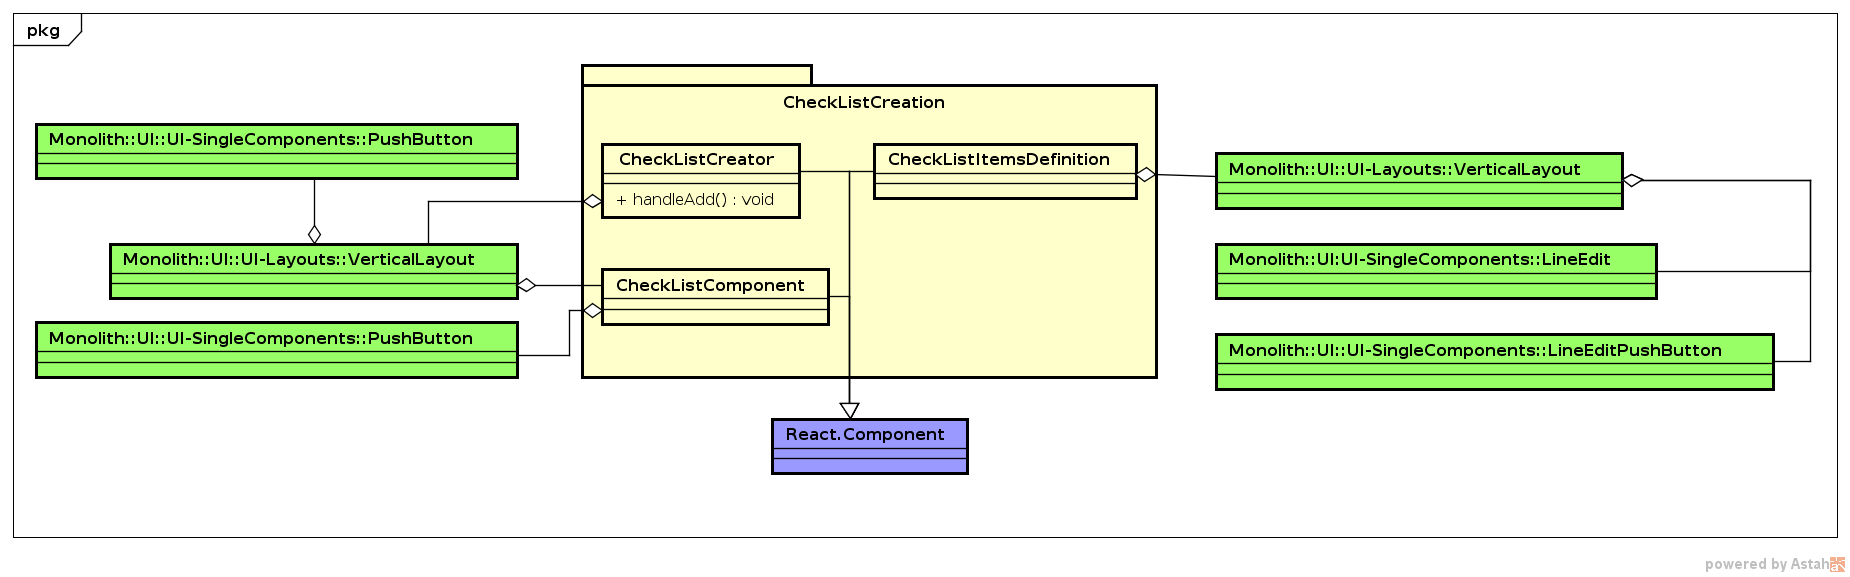
\includegraphics[width=\textwidth,keepaspectratio]{img/listchecklistChecklistCreation}
  \captionof{figure}{Diagramma per ListBubble::CheckListCreation.}
\end{minipage}}
}
%\end{center}
%\end{sidewaysfigure}
\FloatBarrier
\textbf{Descrizione}:\\
 Componente che si occupa della creazione delle check list. 
\\ \textbf{Classi contenute}:\\
\begin{itemize}
\item CheckListComponent
\item CheckListCreator
\item CheckListItemsDefinition
\end{itemize}


\clearpage

\subsubsection{ListBubble::CheckListReading}
   \FloatBarrier
 %  \begin{sidewaysfigure}[ht]
%\begin{center}
 \makebox[\textwidth][c]{
\rotatebox{90}{
% \centering
\begin{minipage}{0.8\textheight}
   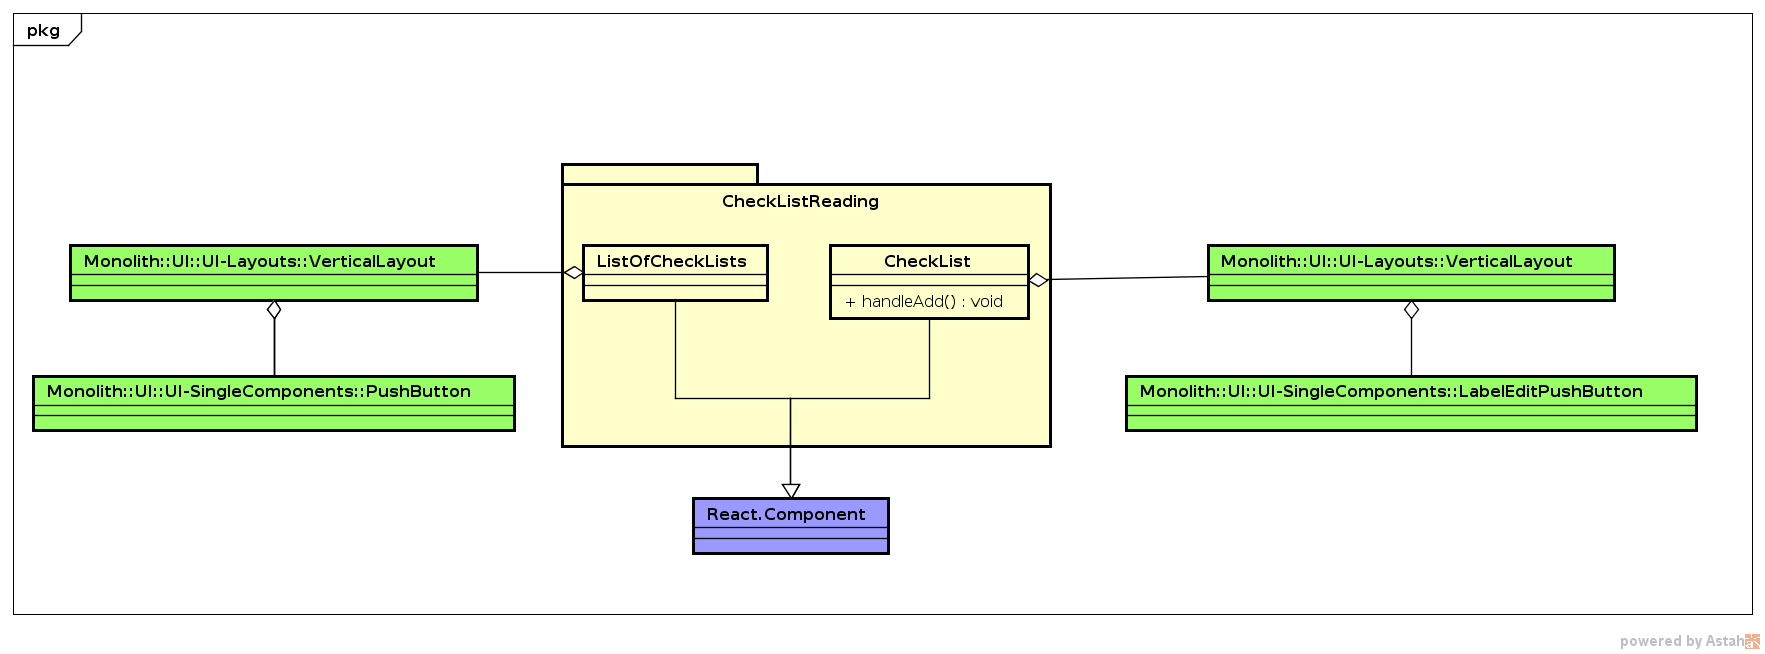
\includegraphics[width=\textwidth,keepaspectratio]{img/listchecklistReading}
  \captionof{figure}{Diagramma per ListBubble::CheckListReading.}
\end{minipage}}
}
%\end{center}
%\end{sidewaysfigure}
\FloatBarrier
\textbf{Descrizione}:\\
 Componente che si occupa della lettura e dell'utilizzo delle check list. 
\\ \textbf{Classi contenute}:\\
\begin{itemize}
\item CheckList
\item ListOfCheckLists
\end{itemize}


\clearpage

\subsubsection{ListBubble::Configuration}
   \FloatBarrier
 %  \begin{sidewaysfigure}[ht]
%\begin{center}
 \makebox[\textwidth][c]{
\rotatebox{90}{
% \centering
\begin{minipage}{0.8\textheight}
   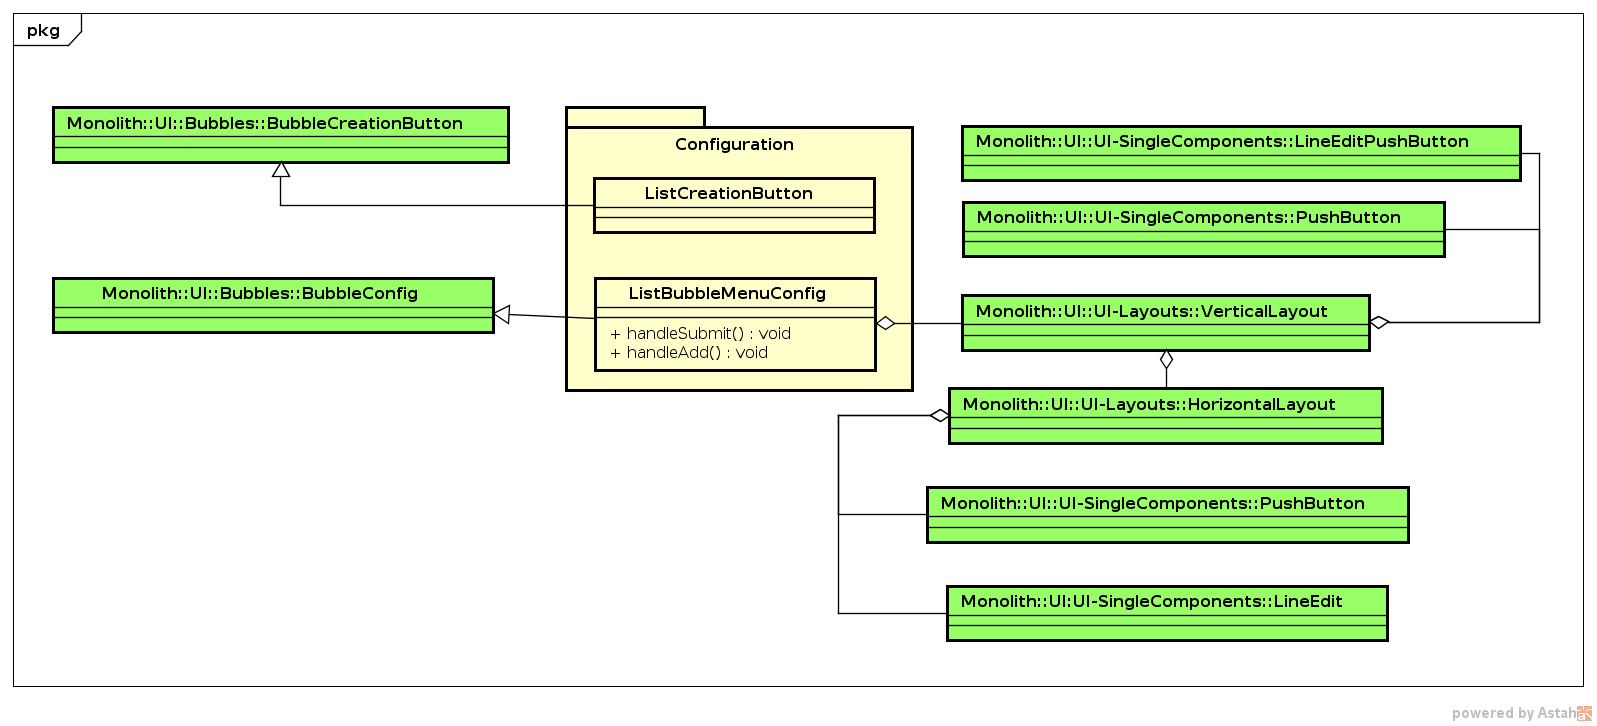
\includegraphics[width=\textwidth,keepaspectratio]{img/listchecklistConfiguration}
  \captionof{figure}{Diagramma per ListBubble::Configuration.}
\end{minipage}}
}
%\end{center}
%\end{sidewaysfigure}
\FloatBarrier
\textbf{Descrizione}:\\
 Componente che gestisce l'area di configurazione della bolla e il pulsante apposito da inserire nel menu iniziale di creazione. 
\\ \textbf{Classi contenute}:\\
\begin{itemize}
\item ListBubbleMenuConfig
\item ListCreationButton
\end{itemize}


\clearpage

\subsubsection{ListBubble::DataManagement}
   \FloatBarrier
   \begin{figure}[ht]
   \centering
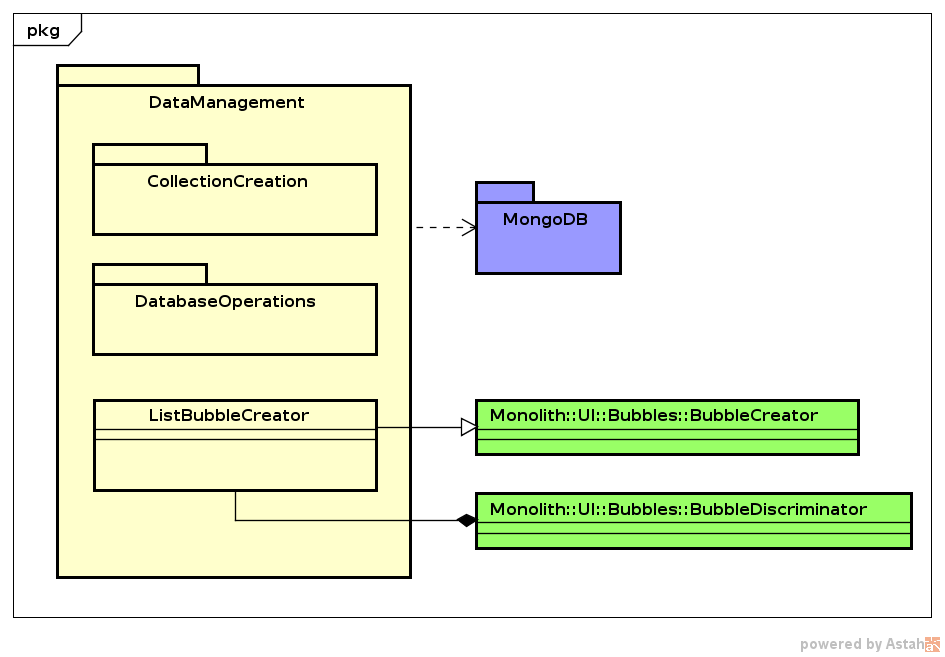
\includegraphics[width=\textwidth,keepaspectratio]{img/listchecklistDatabase}
   \caption{Diagramma per ListBubble::DataManagement.}
\end{figure}
\FloatBarrier
\textbf{Descrizione}:\\
 Componente che si occupa di tutte le operazioni di gestione dei dati che non sono gestite da Monolith. Usa il database MongoDB. 
\\ \textbf{Classi contenute}:\\
\begin{itemize}
\item ListBubbleCreator
\end{itemize}


\clearpage

\subsubsection{ListBubble::Receiver}
   \FloatBarrier
   \begin{figure}[ht]
   \centering
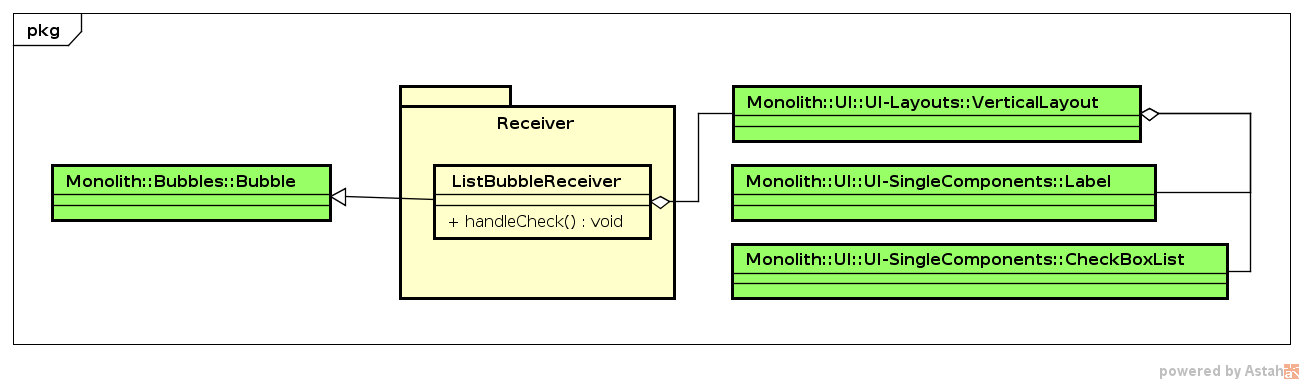
\includegraphics[width=\textwidth,keepaspectratio]{img/listchecklistReceiver}
   \caption{Diagramma per ListBubble::Receiver.}
\end{figure}
\FloatBarrier
\textbf{Descrizione}:\\
 Componente che gestisce la visualizzazione della bolla da parte del ricevente. 
\\ \textbf{Classi contenute}:\\
\begin{itemize}
\item ListBubbleReceiver
\end{itemize}


\clearpage

\subsubsection{ListBubble::Sender}
   \FloatBarrier
 %  \begin{sidewaysfigure}[ht]
%\begin{center}
 \makebox[\textwidth][c]{
\rotatebox{90}{
% \centering
\begin{minipage}{0.8\textheight}
   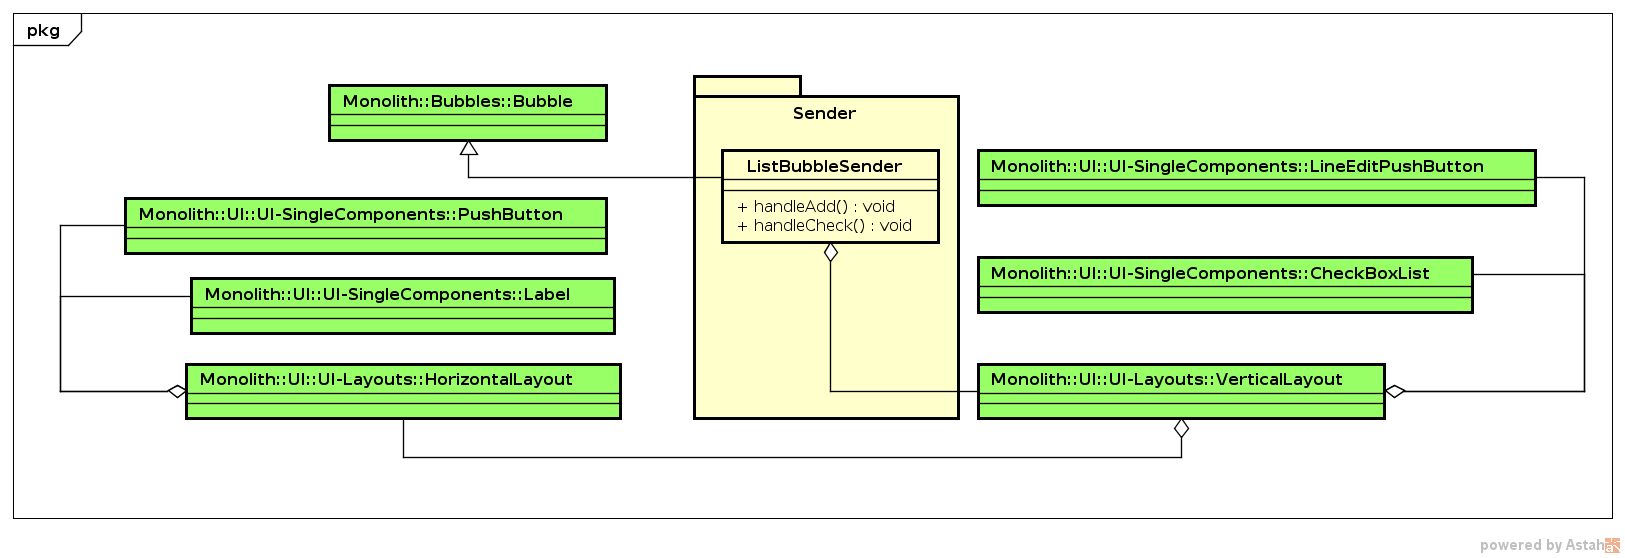
\includegraphics[width=\textwidth,keepaspectratio]{img/listchecklistSender}
  \captionof{figure}{Diagramma per ListBubble::Sender.}
\end{minipage}}
}
%\end{center}
%\end{sidewaysfigure}
\FloatBarrier
\textbf{Descrizione}:\\
 Componente che gestisce la visualizzazione della bolla da parte del mittente. 
\\ \textbf{Classi contenute}:\\
\begin{itemize}
\item ListBubbleSender
\end{itemize}


\clearpage

\subsubsection{MeteoBubble}
   \FloatBarrier
 %  \begin{sidewaysfigure}[ht]
%\begin{center}
 \makebox[\textwidth][c]{
\rotatebox{90}{
% \centering
\begin{minipage}{0.8\textheight}
   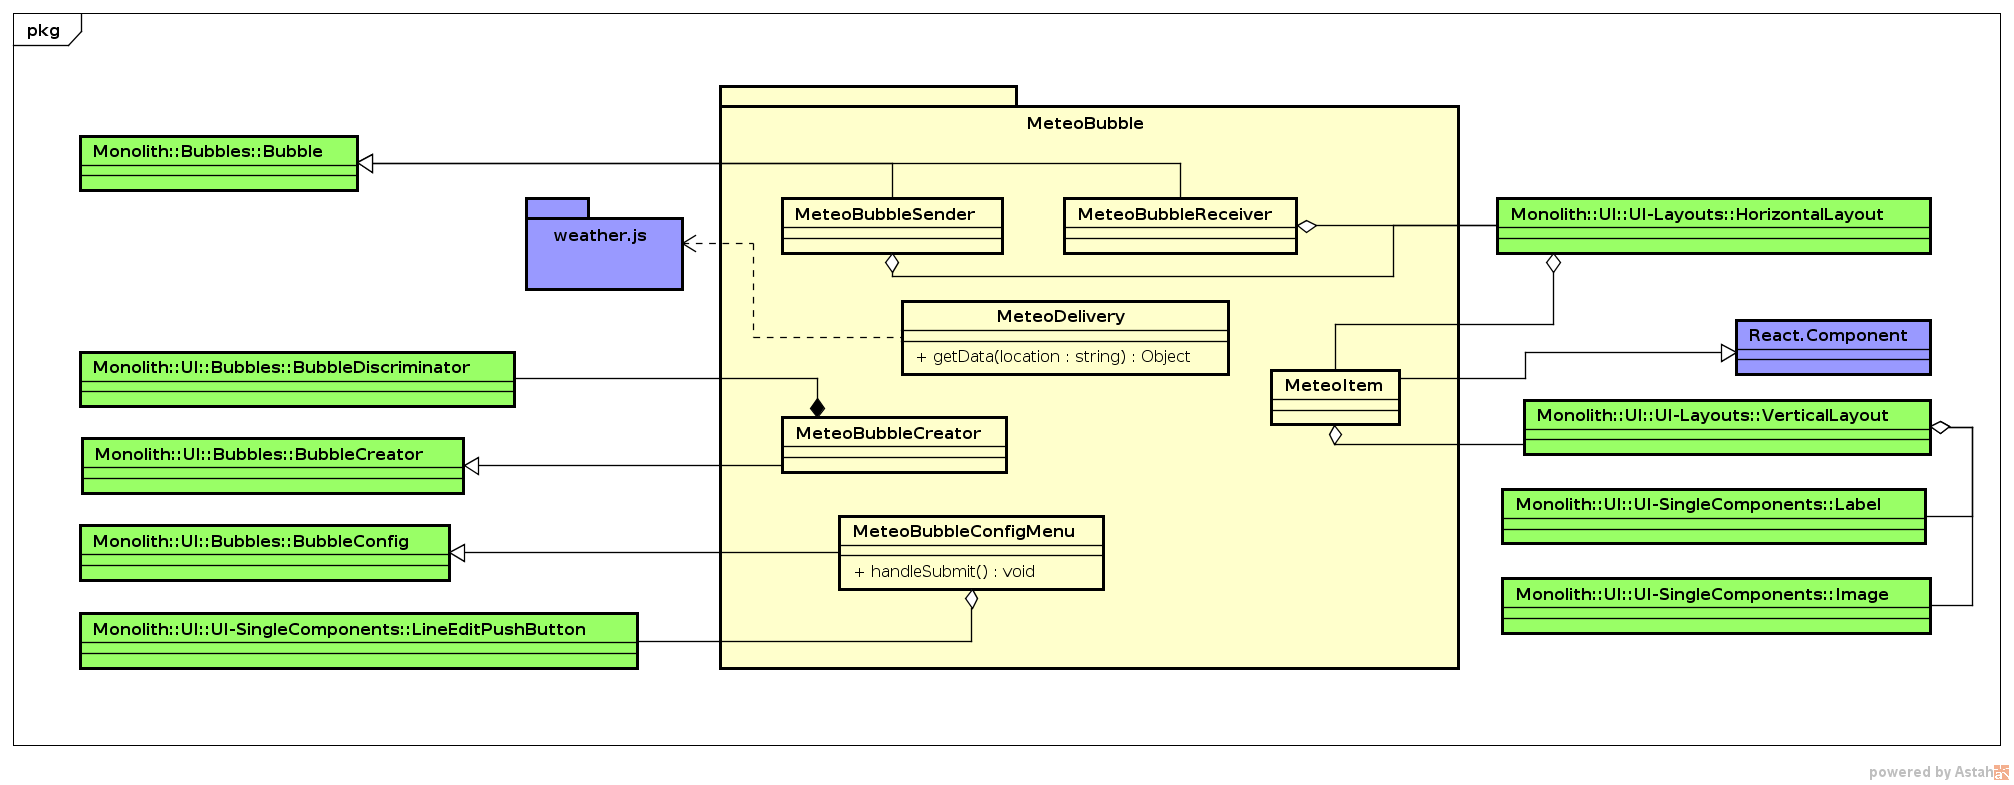
\includegraphics[width=\textwidth,keepaspectratio]{img/meteo}
  \captionof{figure}{Diagramma per MeteoBubble.}
\end{minipage}}
}
%\end{center}
%\end{sidewaysfigure}
\FloatBarrier
\textbf{Descrizione}:\\
 Componente contente le classi necessarie per la creazione della bolla meteo. 
\\ \textbf{Classi contenute}:\\
\begin{itemize}
\item MeteoBubbleConfigMenu
\item MeteoBubbleCreator
\item MeteoBubbleReceiver
\item MeteoBubbleSender
\item MeteoDelivery
\item MeteoItem
\end{itemize}


\clearpage

\subsubsection{SurveyBubble}
   \FloatBarrier
 %  \begin{sidewaysfigure}[ht]
%\begin{center}
 \makebox[\textwidth][c]{
\rotatebox{90}{
% \centering
\begin{minipage}{0.8\textheight}
   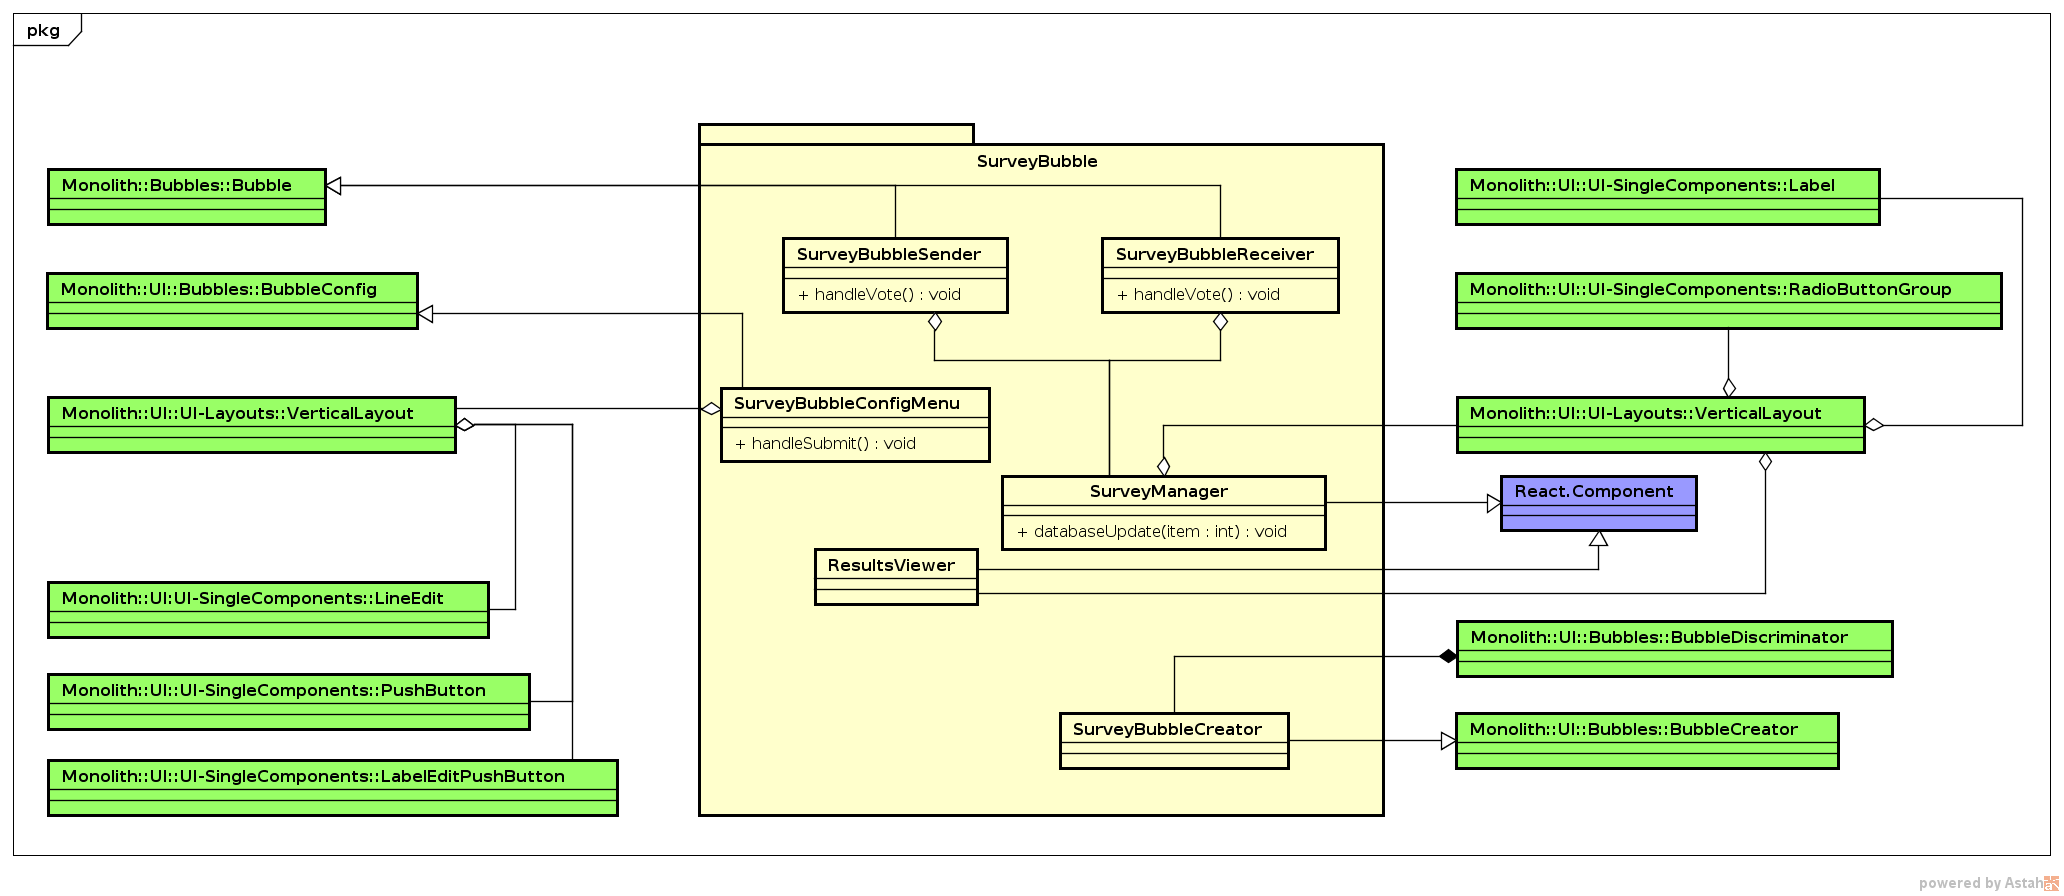
\includegraphics[width=\textwidth,keepaspectratio]{img/survey}
  \captionof{figure}{Diagramma per SurveyBubble.}
\end{minipage}}
}
%\end{center}
%\end{sidewaysfigure}
\FloatBarrier
\textbf{Descrizione}:\\
 Componente contente le classi necessarie per la creazione della bolla sondaggio. 
\\ \textbf{Classi contenute}:\\
\begin{itemize}
\item ResultsViewer
\item SurveyBubbleConfigMenu
\item SurveyBubbleCreator
\item SurveyBubbleReceiver
\item SurveyBubbleSender
\item SurveyManager
\end{itemize}


\clearpage

\subsubsection{TranslationBubble}
   \FloatBarrier
 %  \begin{sidewaysfigure}[ht]
%\begin{center}
 \makebox[\textwidth][c]{
\rotatebox{90}{
% \centering
\begin{minipage}{0.8\textheight}
   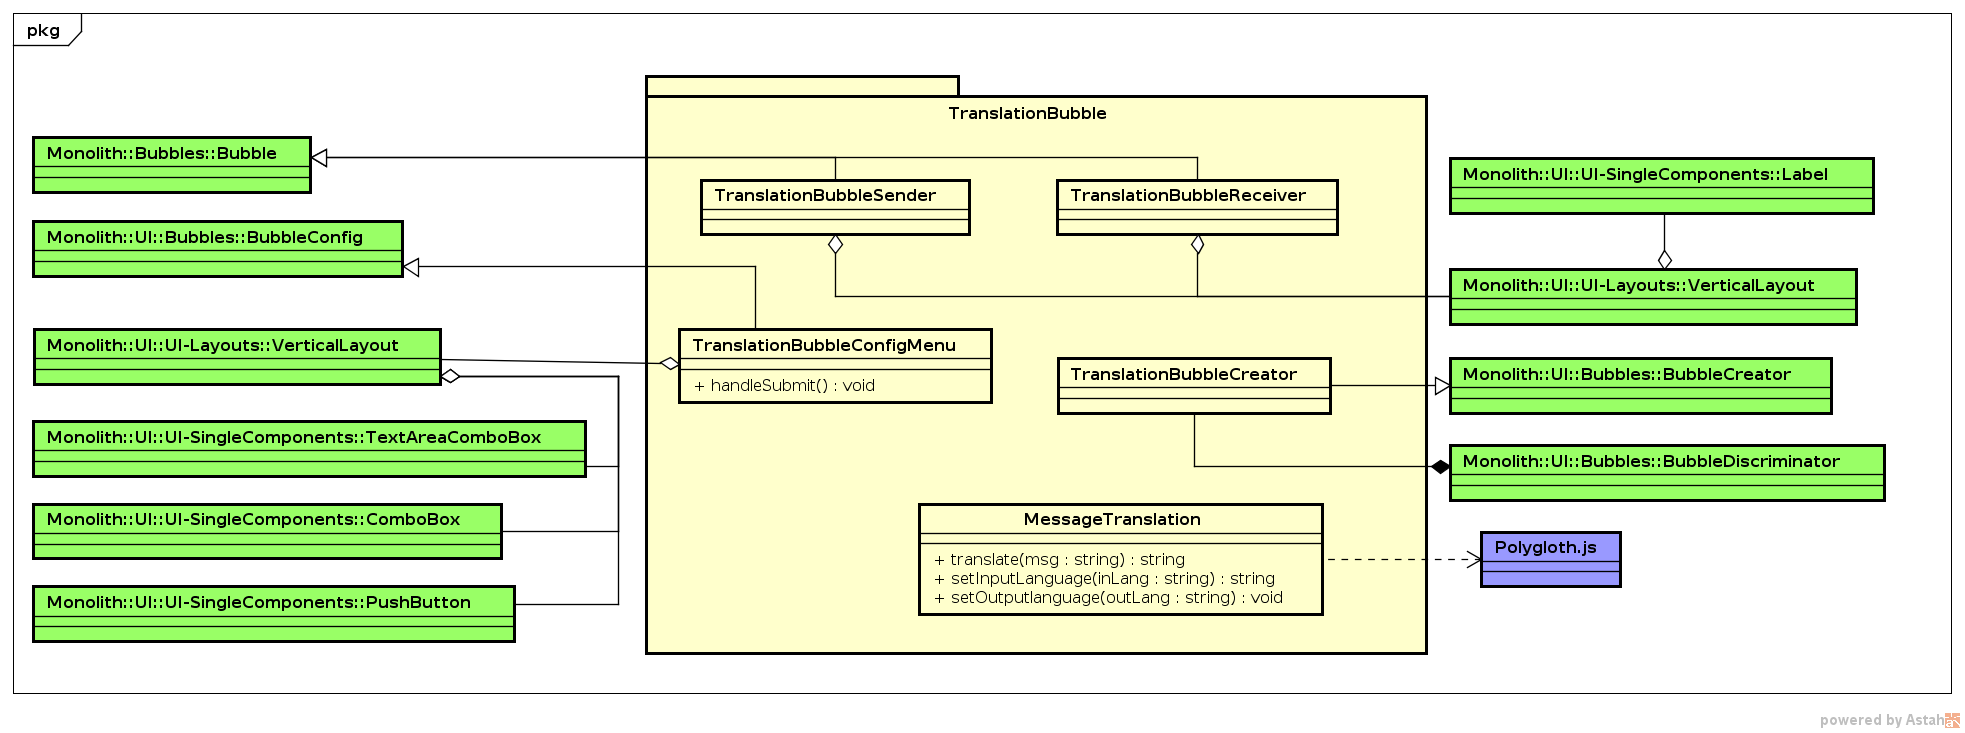
\includegraphics[width=\textwidth,keepaspectratio]{img/translate}
  \captionof{figure}{Diagramma per TranslationBubble.}
\end{minipage}}
}
%\end{center}
%\end{sidewaysfigure}
\FloatBarrier
\textbf{Descrizione}:\\
 Componente contente le classi necessarie per la creazione della bolla traduttore. 
\\ \textbf{Classi contenute}:\\
\begin{itemize}
\item MessageTranslation
\item TranslationBubbleConfigMenu
\item TranslationBubbleCreator
\item TranslationBubbleReceiver
\item TranslationBubbleSender
\end{itemize}


